% article example for classicthesis.sty
\documentclass[10pt,a4paper]{article} % KOMA-Script article scrartcl
\usepackage{import}
\usepackage{xifthen}
\usepackage{pdfpages}
\usepackage{transparent}
\newcommand{\incfig}[1]{%
    \def\svgwidth{\columnwidth}
    \import{./figures/}{#1.pdf_tex}
}
\usepackage{lipsum}     %lorem ipsum text
\usepackage{titlesec}   %Section settings
\usepackage{titling}    %Title settings
\usepackage[margin=10em]{geometry}  %Adjusting margins
\usepackage{setspace}
\usepackage{listings}
\usepackage{amsmath}    %Display equations options
\usepackage{amssymb}    %More symbols
\usepackage{xcolor}     %Color settings
\usepackage{pagecolor}
\usepackage{mdframed}
\usepackage[spanish]{babel}
\usepackage[utf8]{inputenc}
\usepackage{longtable}
\usepackage{multicol}
\usepackage{graphicx}
\graphicspath{ {./Images/} }
\setlength{\columnsep}{1cm}

% ====| color de la pagina y del fondo |==== %
\pagecolor{black}
\color{white}



\begin{document}
    %========================{TITLE}====================%
    \title{{  Apuntes tema 10 AED  }}
    \author{{Rodrigo Castillo}}
    \date{\today}

    \maketitle


     % ====| Loguito |==== %
    
\includegraphics[width=0.1\linewidth]{negro_cara.png}
    %=======================NOTES GOES HERE===================%

    \section{the multivariate normal likelihood}
        \begin{itemize}
            \item {asumamos que $ p \times 1  $  vectores $ X_1 , X_2 , X_3 ,
                ... , X_n  $  represent a random saple from a multivariate
                normal population with mean vector $ \mu  $  and covariance
                matrix
                $ \sigma   $  }
            \item {desde que $ X_1 , X_2 , ... , X_N  $ son mutuamente
                independiente desde una distribución $ N_p(\mu,\sigma )  $  la
            densidad de la funcion converge a normal }
        \end{itemize}

        \begin{itemize}
            \item {cuando los valores numericos de las observacion estan
                disponibles se sustituyen por $ x_j  $ en la ecuacion}
            \item {la expresion resultante ahora se considera en funcion de $
                \mu  $  y $ \sigma   $  para el conjunto arreglado de las
                observaciones $ x_1 , x_2 , ... , x_j  $ }
            \item {algunos procedimientos estadísticos emplean los valores para
                la poblacion del mejor dato observado}
            \item {un dignificado del \color{red} mejor \color{white} es
                explicar el dato observado}
            \item {Un significado de la mejor forma de seleccionar los valores
                del parametro que maximizan la densidad de la union evaluada en
                    las observaciones se llama el \color{blue} metodo de maxima
                    verosimilitud \color{white}  que maximiza el parametro que se llama
                \color{blue} estimador de maxima verosimilitud \color{white} }
        \end{itemize}

        tenemos que considerar el la estimación de maxima verosimilitud para
        los parametros $ \mu  $  y $ \sigma   $  para una cosa normal
        multivariada
        \\ para hacer esto, vamos a tener que tomar las observaciones $ x_1 ,
        x_2 , ... , x_n  $ como arreglos

        \begin{figure}[h!]
            \centering
            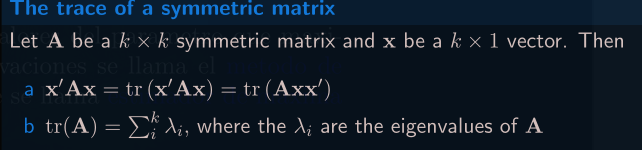
\includegraphics[width=0.8\linewidth]{mle.png}
            \caption{MLE OBSERVATIONS}
            \label{shit fuck i hate this shit pls anyone kill me}
        \end{figure}

    \section{maximum likelihood estimation of $ \mu  $  and $ \sigma   $ }

        \begin{figure}[h!]
            \centering
            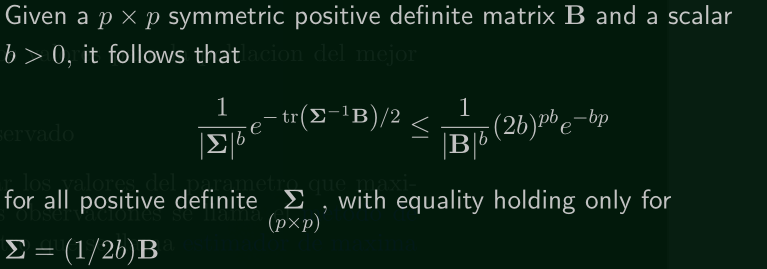
\includegraphics[width=0.8\linewidth]{mle2.png}
            \caption{MLE of $ \mu  $ y $ \sigma   $ }
            \label{fig}
        \end{figure}

        \begin{figure}[h!]
            \centering
            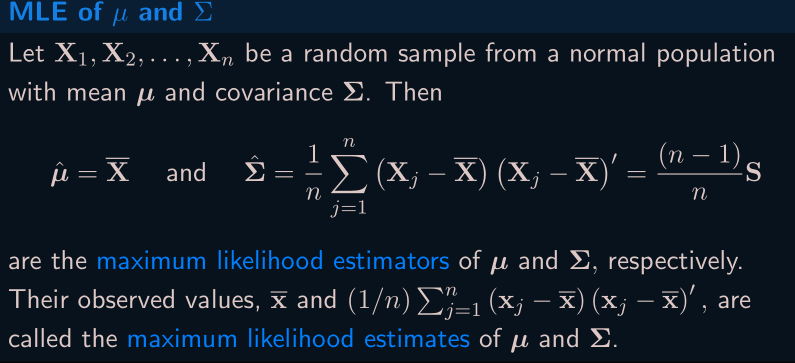
\includegraphics[width=0.8\linewidth]{mle3.png}
            \caption{MLE definiciojes}
            \label{kill me}
        \end{figure}




    \section{the sampling distribution of $ \hat{X}   $  and $ S  $ }
        consideraciones:

        \begin{figure}[h!]
            \centering
            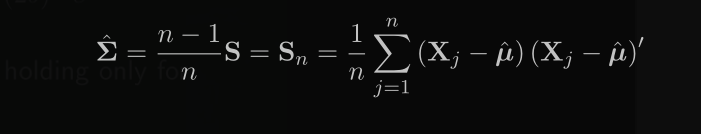
\includegraphics[width=0.8\linewidth]{form.png}
            \caption{estimadores para $ \mu  $  y $ \sigma  $  }
            \label{fig}
        \end{figure}


    \section{Large-Sample Behavior of $ \hat{X}   $ and $ S  $ }
        \begin{figure}[h!]
            \centering
            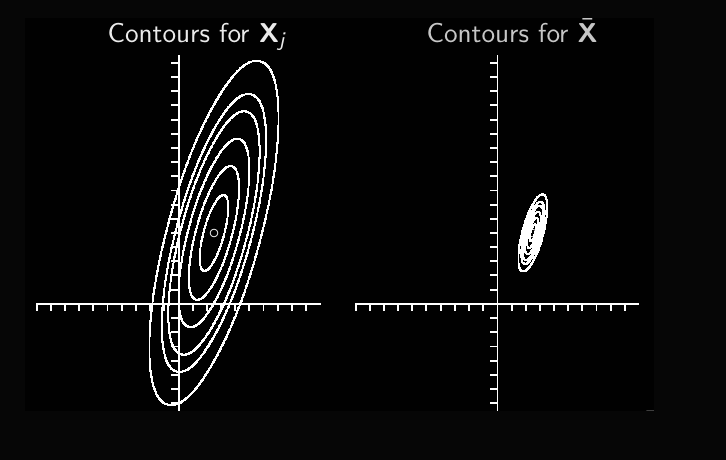
\includegraphics[width=0.8\linewidth]{beh.png}
            \caption{Comportamiento}
            \label{duque está llorando jaja}
        \end{figure}






















    %=======================NOTES ENDS HERE===================%

    % bib stuff
    \nocite{*}
    \addtocontents{toc}{{}}
    \addcontentsline{toc}{section}{\refname}
    \bibliographystyle{plain}
    \bibliography{../Bibliography}
\end{document}
